\chapter{Problem Definition}

Given one or more  in the shopping cart the problem statement is to suggest items complementary to it which may contain garments or accessories which makes a complete set as per current fashion.

Physically speaking if someone adds a top in her shopping cart, we try to suggest her matching/complementary jeans, denim, skirt, bag, sunglasses, shoes, etc. which go well with the product chosen and make a complete set of items that can be used together.


\begin{figure}[htb]
\centering
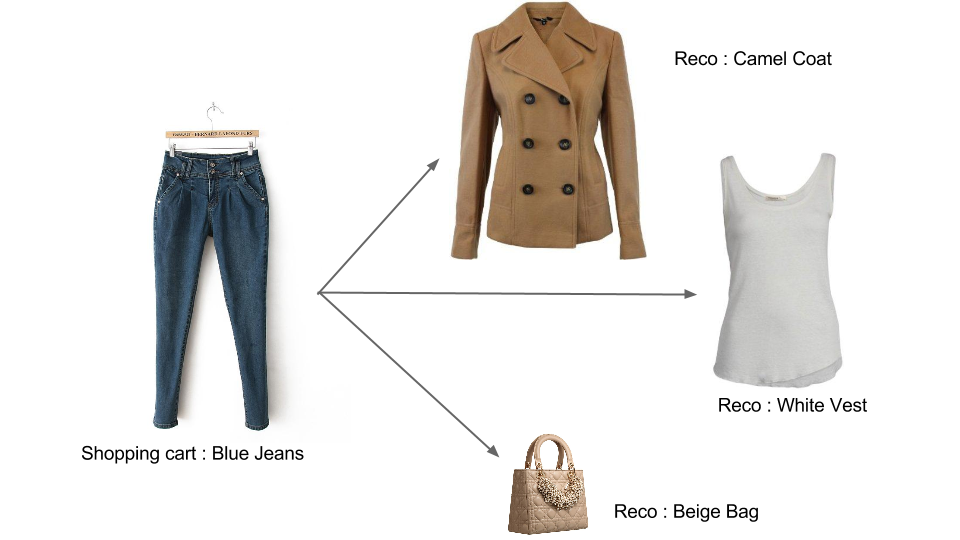
\includegraphics[scale=0.4]{Untitled} % e.g. insert ./image for image.png in the working directory, adjust scale as necessary
\caption{Problem Definition: Complete the look recommendation}
\label{fig:introPic} % insert suitable label, this is used to refer to a fig from within the text as shown above
\end{figure}
